\documentclass[12pt,letterpaper]{article}
\usepackage[UTF8]{ctex}
\usepackage{fullpage}
\usepackage[top=2cm, bottom=4.5cm, left=2.5cm, right=2.5cm]{geometry}
\usepackage{amsmath,amsthm,amsfonts,amssymb,amscd}
\usepackage{lastpage}
\usepackage{enumerate}
\usepackage{fancyhdr}
\usepackage{mathrsfs}
\usepackage{xcolor}
\usepackage{graphicx}
\usepackage{listings}
\usepackage{hyperref}
\usepackage{dot2texi}
\usepackage{tikz}
\usepackage{float}
\usepackage[pdf]{graphviz}
\usetikzlibrary{automata,shapes,arrows} 

\hypersetup{%
  colorlinks=true,
  linkcolor=blue,
  linkbordercolor={0 0 1}
}
 
\renewcommand\lstlistingname{Algorithm}
\renewcommand\lstlistlistingname{Algorithms}
\def\lstlistingautorefname{Alg.}

\lstdefinestyle{Matlab}{
    language        = matlab,
    frame           = lines, 
    basicstyle      = \footnotesize,
    keywordstyle    = \color{blue},
    stringstyle     = \color{green},
    commentstyle    = \color{red}\ttfamily
}
\setlength{\parindent}{0.0in}
\setlength{\parskip}{0.05in}

% Edit these as appropriate
\newcommand\course{自然语言处理基础}
\newcommand\hwnumber{1}                  % <-- homework number
\newcommand\name{张东方}                 % <-- Name
\newcommand\ID{2100013521}           % <-- ID

\pagestyle{fancyplain}
\headheight 35pt
\lhead{\name\\\ID}                 
\chead{\textbf{\Large Homework \hwnumber}}
\rhead{\course \\ \today}
\lfoot{}
\cfoot{}
\rfoot{\small\thepage}
\headsep 1.5em





\begin{document}

\section*{1.数据预处理}
  我发现数据中有一些词后面连着特殊符号,如"-"、"\textbackslash"、"/"、"\&"等。这些符号充当分隔符,因此我将它们全部替换成空格。比如,"high-quality"被替换成"high quality","and/or"被替换成"and or"。我将所有数字替换成\verb|<|NUM\verb|>|。在此过程中,我发现有些数字紧连着单词,如"10ml"。为了便于后续分词,我在所有数字前后都加上空格,如"10 ml"。我按空格分割所有词汇,并将它们存到一个list里。为了节省空间,我将原始数据的title和description列合在一块,丢掉了原来的这两列。接着,我将所有词都转换为小写形式,去除了's后缀,并去除了所有标点符号,包括[.,:()'"?;\#\verb|$|!]。我使用了nltk库提供的英文停用词表。但我保留了表中表示单位的词,如s、m等,并额外添加了"--"、""等特殊符号作为停用词。我使用了nltk库提供的WordNetLemmatizer进行词形还原,将所有词还原到其基本形式。为了避免重复计算,我将处理后的数据保存为一个pkl文件。

\section*{2.特征提取}

我使用字典统计每个词在所有文档中出现的总次数。其中,词作为字典的key,次数作为对应的value。基于这个字典,我可以计算每个词的IDF值。对于每个文档,我统计其中每个词出现的次数,计算TF值。将每个词的TF值和IDF值相乘,得到该词在该文档中的TF-IDF值。考虑到文本数据的高维稀疏特性,我使用了scipy库提供的csr\_matrix,以压缩稀疏行矩阵的形式存储所有文档的TF-IDF值。

\section*{3.构建Log-Linear模型并训练}
在这一部分,我构建并训练了一个Log-Linear模型。首先,我使用sklearn库的train\_test\_split函数,按照8:2的比例随机划分训练集和评估集。

为了便于模型训练,我将标签列(共4个类别)展开成one-hot形式。这样,标签就变成了一个二维矩阵,每一行对应一个文档,每一列对应一个类别。这种表示方式便于后续的矩阵运算。

在模型初始化时,我将权重矩阵初始化为一个标签数*特征数的零矩阵。然后,我使用随机梯度下降法对模型进行训练。本来我想使用课件上的线搜索方法进行训练,但在训练阶段发现过于缓慢,因此改用随机森林。

在每个训练epoch时,我首先打乱训练数据的顺序,然后按批次进行迭代。在每个批次中,我首先提取该批次对应的tf-idf子矩阵,并与权重矩阵的转置进行矩阵乘法,得到每个样本在不同类别下的分数。接着,我对这些分数应用softmax函数,得到预测的概率分布。

为了计算损失,我将预测的概率分布与真实的one-hot标签相减,得到误差delta。然后,我将误差矩阵的转置与该批次的tf-idf子矩阵相乘,得到梯度矩阵。最后,我将梯度矩阵乘以学习率,并从当前的权重矩阵中减去,以更新权重。

经过多个epoch的训练后,我将训练好的模型保存为一个pkl文件,以便后续的加载和使用。在训练过程中,我使用了0.01的学习率,batch大小为128,训练了100个epoch。这些超参数是通过几次试验和观察训练集和评估集上的损失变化曲线来调优的。

\section*{4.评估与测试}
在预测阶段,我首先将待预测的tf-idf矩阵与训练好的权重矩阵的转置进行点乘操作。这个操作会为每个文档生成一个分数向量,向量的每个元素表示该文档属于相应类别的得分。将这些分数向量传入softmax函数。softmax函数会将分数向量转化为概率分布,使得每个元素都在0到1之间,并且所有元素的和为1。这个过程可以理解为将原始的分数归一化,得到每个类别的概率。使用NumPy的argmax函数找出概率最高的类别,将其作为预测的标签。这样得到了一个预测标签的向量,每个元素对应一个文档的预测类别。将预测的标签向量与真实的标签向量进行比较,计算模型的准确率和F1分数。

在评估集上准确率为0.8732,F1分数为0.8733,使用sklearn的评估工具给出的结果如下:

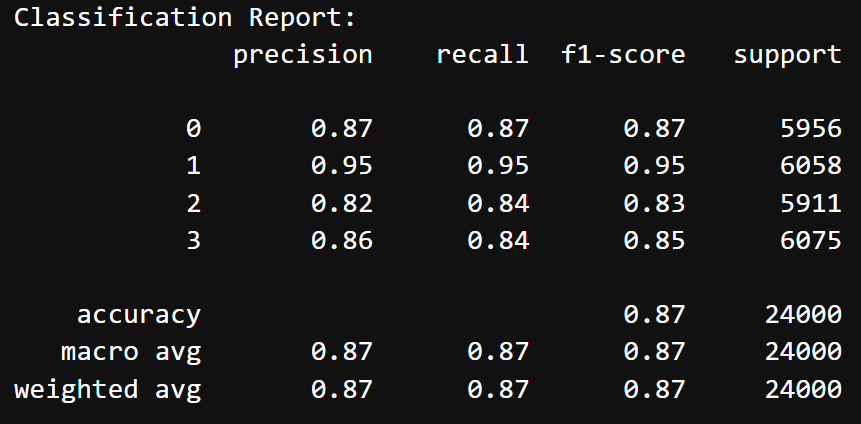
\includegraphics[scale=0.8]{1.png}

在测试集上准确率为0.8043,F1分数为0.8032,使用sklearn的评估工具给出的结果如下:

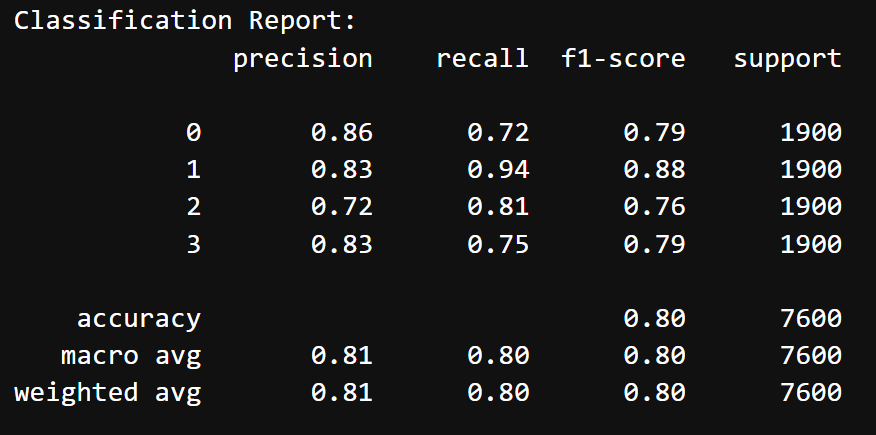
\includegraphics[scale=0.8]{2.png}

\end{document}
